\documentclass[a4paper,12pt]{article}
\usepackage[hmargin=2.5cm,vmargin=2.5cm]{geometry}

\usepackage[utf8]{inputenc}   % le fichier .tex est en UTF-8     
\usepackage[francais]{babel}  %typo française                    
\usepackage[T1]{fontenc}      % encodage des fonts latex         
\usepackage{lmodern}                                             
\usepackage{microtype}        % typo supplémentaires             


\usepackage{multirow}  %  pour des tableaux multilignes/multicolonnes

\usepackage{graphicx} %inclusion de graphiques

\usepackage{hyperref} % liens dans le pdf
\hypersetup{%
  pdftitle={Title},
  pdfauthor={Author1, Author2},
  pdfkeywords={keywords}
  pdfsubject={article},
  colorlinks=true,
  linkcolor=black,
  urlcolor=black,
  citecolor=black
}


\begin{document}

   \begin{figure}[t]
     \centering
     \begin{tabular}{cc}
       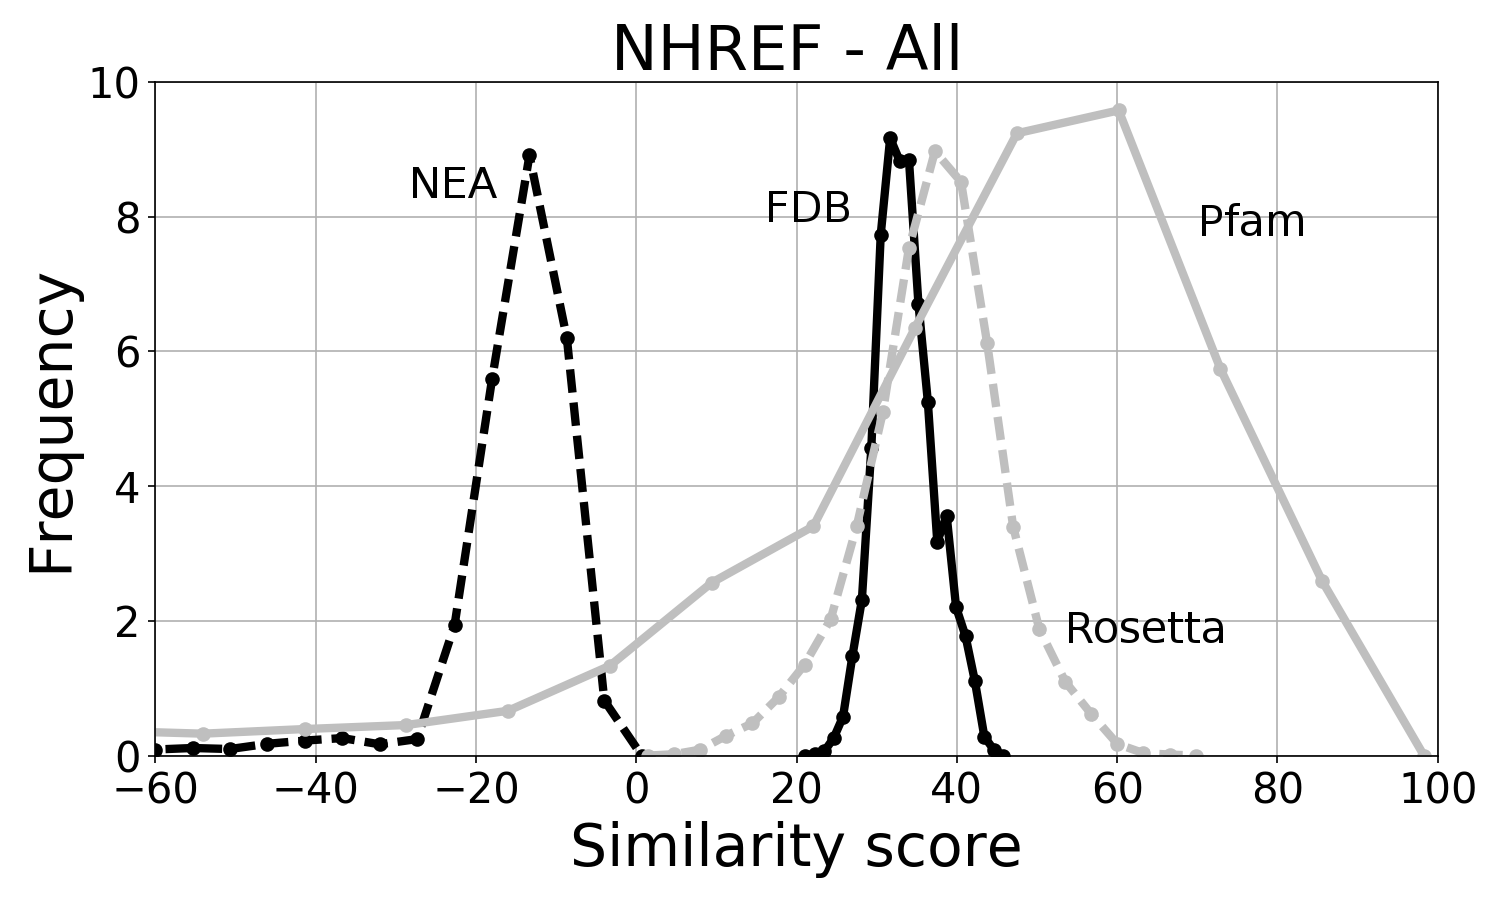
\includegraphics[width=8.4cm]{rapport/resultats/PDZ/graphe/exactGB/1G9O_simil_cut.png} &
       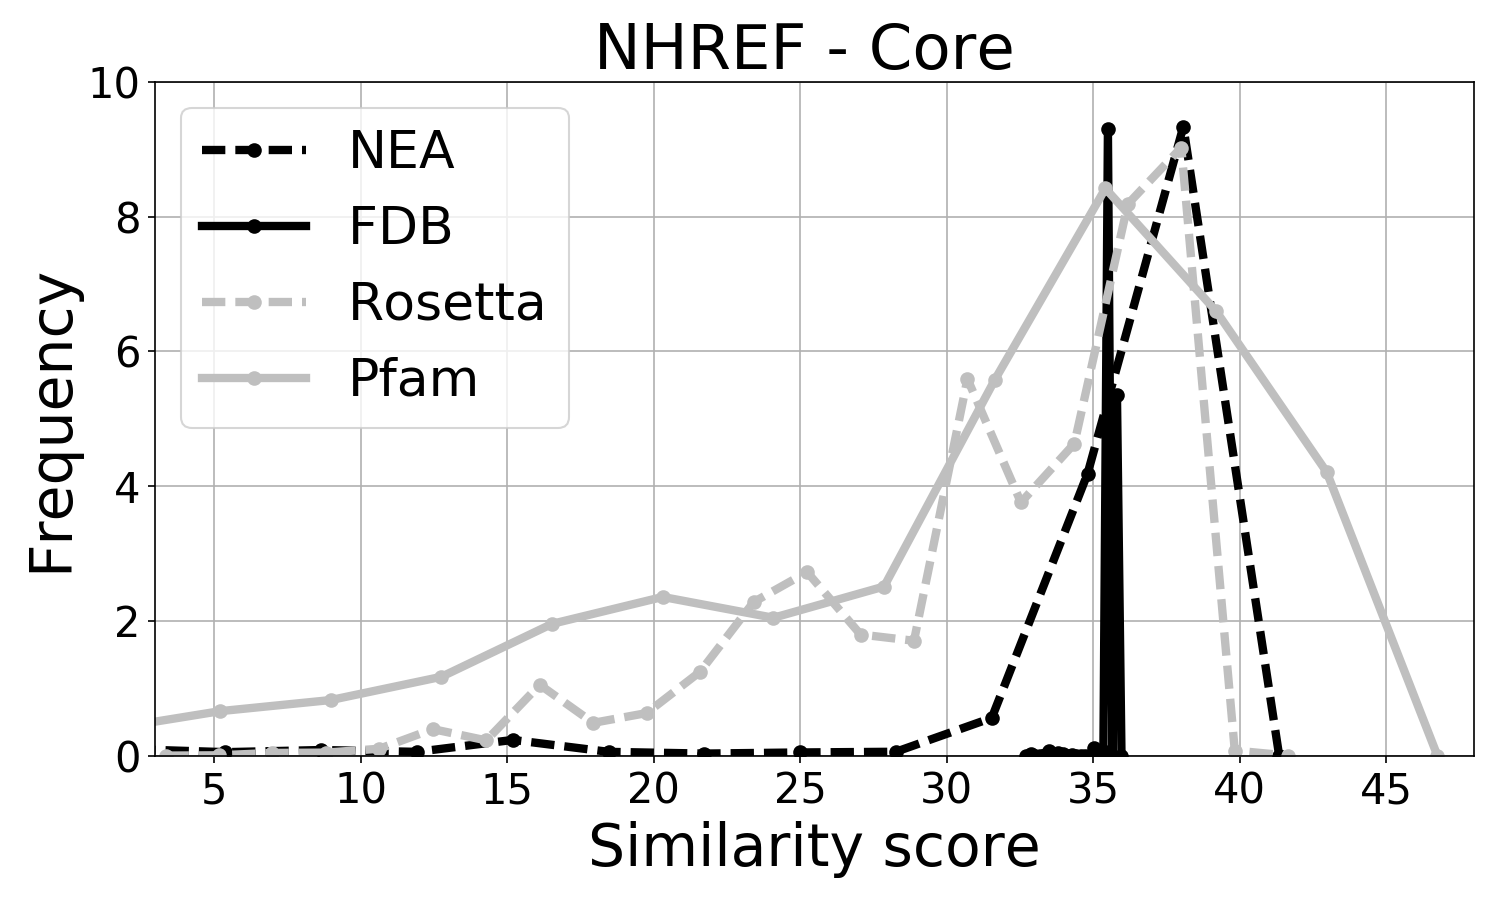
\includegraphics[width=8.4cm]{rapport/resultats/PDZ/graphe/exactGB/1G9O_simil_core.png} \\
       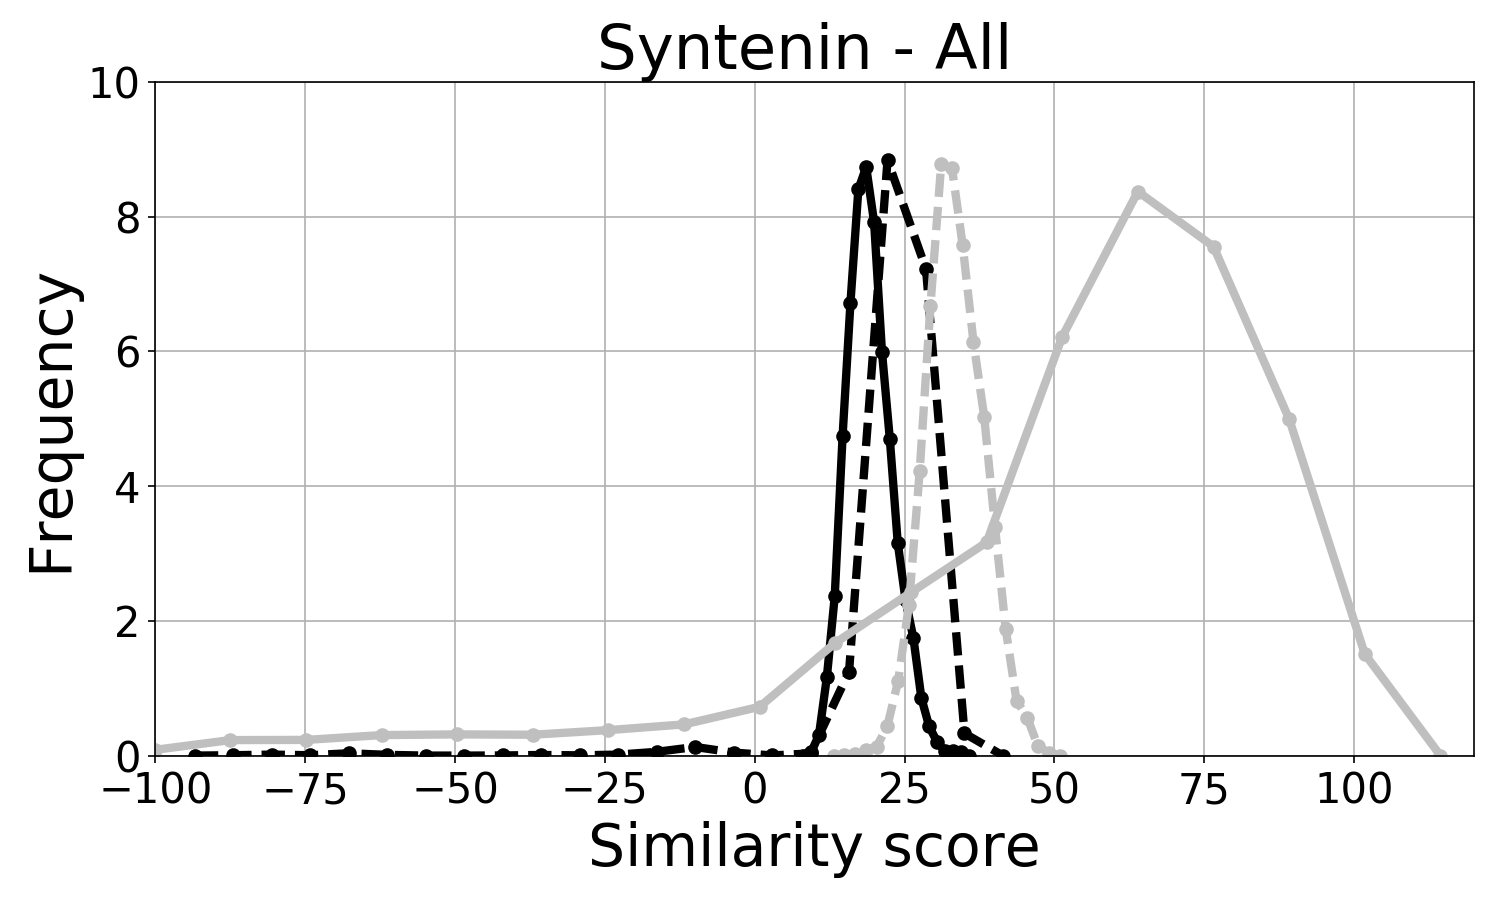
\includegraphics[width=8.4cm]{rapport/resultats/PDZ/graphe/exactGB/1R6J_simil_cut.png} &
       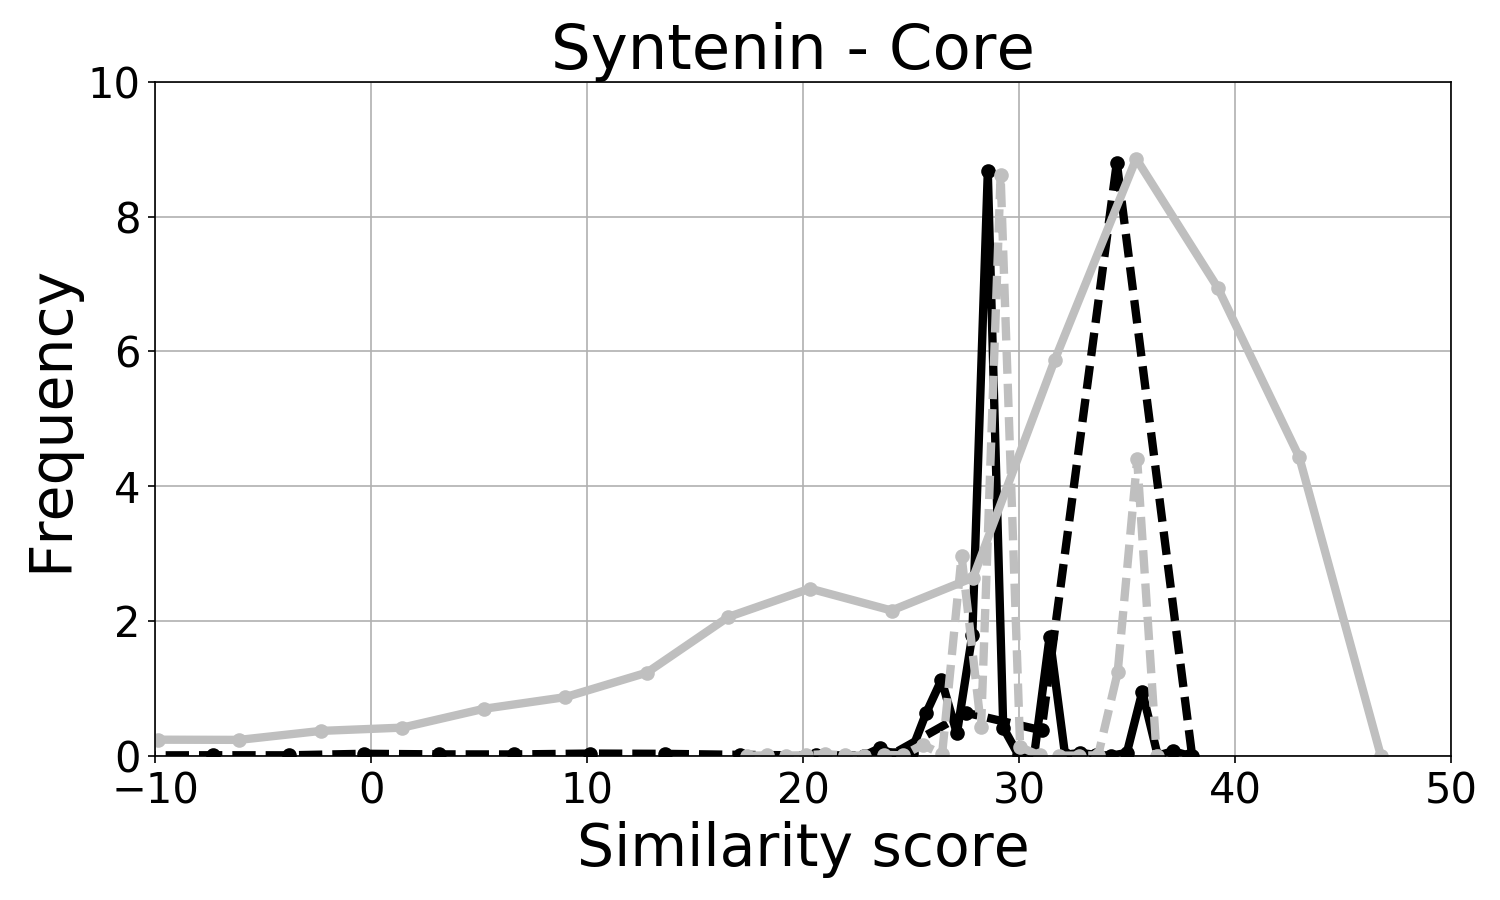
\includegraphics[width=8.4cm]{rapport/resultats/PDZ/graphe/exactGB/1R6J_simil_core.png} \\
       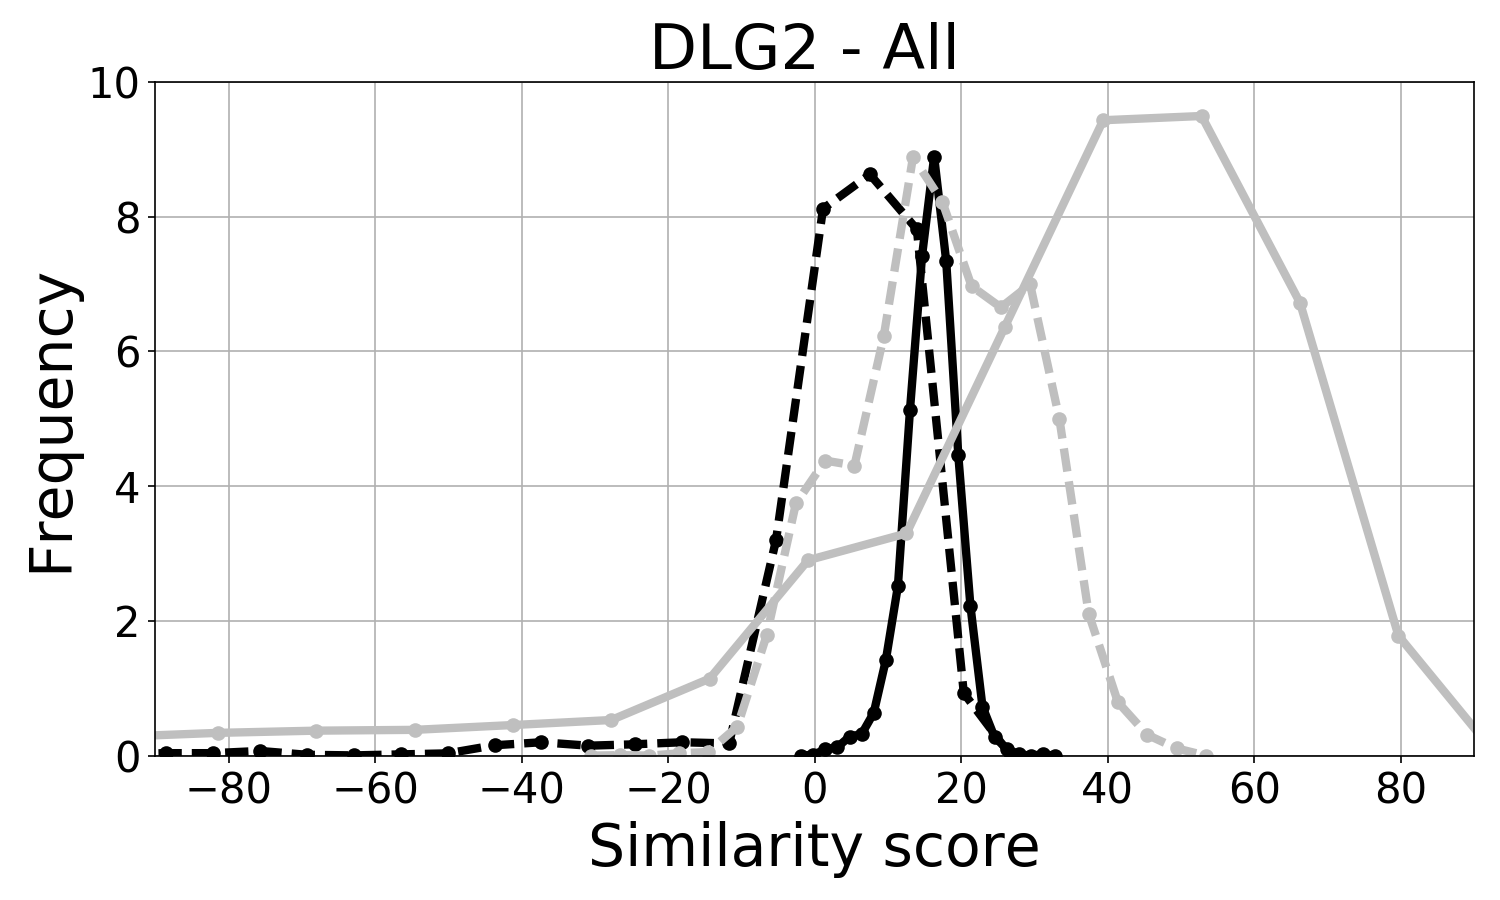
\includegraphics[width=8.4cm]{rapport/resultats/PDZ/graphe/exactGB/2BYG_simil_cut.png} &
       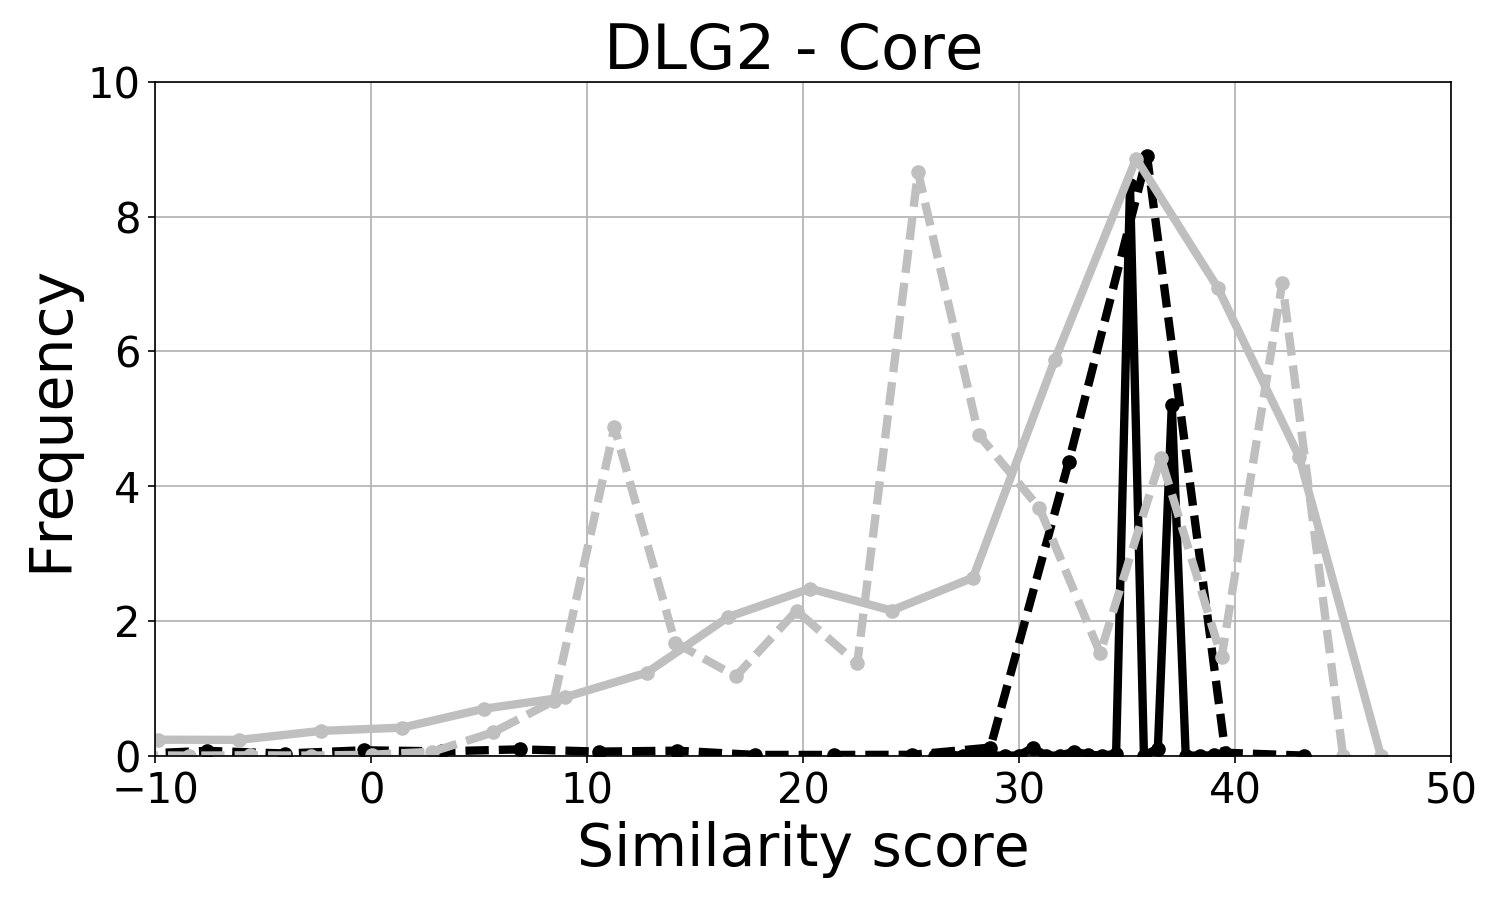
\includegraphics[width=8.4cm]{rapport/resultats/PDZ/graphe/exactGB/2BYG_simil_core.png} \\
     \end{tabular}
\label{graph:Simil_Proteus_PDZ}
   \end{figure}
\thispagestyle{empty}

\end{document}
 

